\documentclass[10pt]{article}
\usepackage{enumitem}
\usepackage{hyperref}
\hypersetup{
	colorlinks=true,
	linkcolor=blue,
	filecolor=magenta,      
	urlcolor=cyan,
}
\usepackage{graphicx}
\usepackage{amsmath}
\usepackage[utf8]{inputenc}
\usepackage{mathtools}
\usepackage[caption=false]{subfig}
\usepackage{soul}
\usepackage[top=0.75in, bottom=0.75in, left=0.5in, right=0.5in]{geometry}
\usepackage[margin=1.5cm]{caption}
\usepackage{epsfig,amsmath}
\DeclarePairedDelimiter\abs{${\lvert}$}{${\rvert}$}%
\usepackage{titlesec,color}
\usepackage{kpfonts}
\usepackage{empheq}
\usepackage{palatino}
\usepackage{graphicx,wrapfig}
\setlength{\parskip}{1em}
\setlength{\parindent}{0pt}
\usepackage{array}
\usepackage{gensymb}
\usepackage{soul}
\usepackage{grffile}
\usepackage{listings}
\usepackage{color}
\usepackage{tcolorbox}
\usepackage{courier}
\usepackage[T1]{fontenc}
\usepackage{helvet}
\usepackage{multicol}
\usepackage[super,sort&compress]{natbib}
\setlength\columnsep{0.3in}
\setlength{\parindent}{1cm}
\setlength{\parskip}{1mm}
\tcbuselibrary{listings,skins}
\tolerance=1
\emergencystretch=\maxdimen
\hyphenpenalty=10000
\hbadness=1000
\hypersetup{citecolor=black}

\definecolor{dkgreen}{rgb}{0,0.6,0}
\definecolor{gray}{rgb}{0.5,0.5,0.5}
\definecolor{mauve}{rgb}{0.58,0,0.82}

\usepackage{titlesec}
\titleformat{\subsection}
  {\normalfont\fontfamily{phv}\fontsize{11}{11}\selctfont}{\thesubsection}{1em}{}

\begin{document}
	
\renewcommand*\rmdefault{phv}
\fontfamily{phv}\selectfont

\newcommand{\avg}[1]{\left<{#1}\right>}
\newcommand{\hence}{\hspace{1cm}\Longrightarrow\hspace{1cm}}
\renewcommand{\ni}{\noindent}
\newcommand{\din}{\indent \indent}
\newcommand{\mni}{\medskip \noindent}
\newcommand{\bni}{\bigskip \noindent}
\newcommand{\sni}{\smallskip \noindent}
\newcommand{\pr}{{\rm Prob}}
\newcommand{\mon}{\begin{displaymath}}
\newcommand{\moff}{\end{displaymath}}
\newcommand{\sumi}[1]{\sum_{{#1}=-\infty}^{\infty}}
\renewcommand{\b}[1]{\mbox{\boldmath ${#1}$}}
\newcommand{\sumy}{\sum_{\b{y}}}
\newcommand{\sumz}{\sum_{\b{z}}}
\newcommand{\pd}[2]{\frac{\partial {#1}}{\partial {#2}}}
\newcommand{\od}[2]{\frac{d {#1}}{d {#2}}}
\newcommand{\odat}[3]{\left. \frac{d {#1}}{d {#2}} \right|_{#3}}
\newcommand{\inti}{\int_{-\infty}^{\infty}}
\newcommand{\eon}{\begin{equation}}
\newcommand{\eoff}{\end{equation}}
\newcommand{\eaon}{\begin{eqnarray}}
\newcommand{\eaoff}{\end{eqnarray}}
\newcommand{\e}[1]{\times 10^{#1}}
\newcommand{\chem}[2]{{}^{#2} \mathrm{#1}}
\renewcommand{\sb}{s}
\newcommand{\s}{s}
\newcommand{\zetaexp}{\left( \zeta e^{q \s t} \right)}
\newcommand{\taunuc}{\tau_{nuc}}
\newcommand{\eq}[1]{Eq. (\ref{#1})}\
\newcommand{\ev}[1]{\langle #1 \rangle}
\newcommand*\mean[1]{${\bar{#1}}$}
\newcolumntype{L}{>{\centering\arraybackslash}m{5cm}}
\bibliographystyle{unsrtnat}


\vspace*{\stretch{1.0}}
\begin{center}
	\LARGE\textbf{MARGO (Massively Automated Real time GUI for Object-tracking), a platform for high-throughput ethology}\\
	\large\textbf{}
\end{center}
\vspace*{\stretch{2.0}}
\rightline{\textbf{Zach Werkhoven}, \textbf{Chuan Qin}, \textbf{Christian Rohrsen}, \textbf{Björn Brembs}, \textbf{Benjamin de Bivort}}
\rightline{\small Dept. of Organismic and Evolutionary Biology, Harvard University, Cambridge MA, 02138}
\rightline{\small Institut für Zoologie - Neurogenetik, Universität Regensburg, Regensburg, Germany}

\section*{Abstract}

Automated animal tracking offers the potential to probe the mechanisms underlying behavior more deeply than comparable manual approaches. Fast tracking in real time allows convenient tracking of very large numbers of animals or conducting experiments that require closed-loop stimulus control for multiple animals in parallel. We developed MARGO, a real time animal tracking suite for conducting custom behavioral experiments. We demonstrated that MARGO can rapidly and accurately track large numbers of animals in parallel. We show that MARGO's robustness to changes in image background and tracking speed make it feasible to tracking large cohorts of animals over very long timescales. Additionally, we incorporated control of peripheral hardware, and implemented a convenient software architecture for defining new experimental routines. These features enable closed-loop delivery of stimuli to many individuals simultaneously. We highlight MARGO's ability to tightly coordinate tracking and hardware control in parallel with two custom behavioral assays (measuring phototaxis and optomotor response). There are currently several open source software packages for animal tracking. MARGO’s strength is being a flexible platform with the potential to accelerate a wide-variety of behavioral experiments and bring sophisticated stimulus control to the realm of large-scale experimentation and screening.

\vspace{1cm}
\begin{multicols}{2}
\section*{Introduction}

Automated animal tracking methods have become commonplace in the study of behavior. They enable large sample sizes, high statistical power, and more rapid inference of the various mechanisms giving rise to behavior. Existing animal trackers vary in computational complexity and specialization to particular imaging configurations. In part, tracker diversity can be attributed to the diversity of desired behavioral measurements. Trackers can assist in a wide range of experimental tasks such as monitoring activity, measuring response to stimuli\cite{Fry_TrackFly_2008,Donelson_High_2012}, and recording postural changes over time\cite{Mathis_DeepLabCut_2018,Pereira_Fast_2018}. Some trackers are designed to track and maintain identities of multiple individuals occupying the same arena \cite{Prez-Escudero_idTracker_2014,Eyjolfsdottir_Detecting_2014,Rodriguez_ToxId_2017} while others measure the collective activity of groups without maintaining identities or rely on physical segregation of animals to ensure trajectories never collide \cite{Ramot_The_2008,Swierczek_High_2011,Itskovits_A_2017}. But few of these trackers are designed as platforms for high throughput, hardware control, and flexible experimental reconfiguration. 

Improvements in machine learning and template matching approaches to object localization and classification have made it possible to efficiently train models that accurately track and classify a variety of animal species and visually distinguish identities of individuals across time \cite{Eyjolfsdottir_Detecting_2014,Prez-Escudero_idTracker_2014}. Tracking individual identity in groups requires resolving identities through collisions where bodies are overlapping. Tracking applications idTracker and FlyTracker train classifiers to assign identities to individuals in each frame and can also be used to extract postural information such head and limb position. When trained well, these trackers can maintain distinct identities over extended periods with minimal human intervention. Other applications, such as Ctrax and Tracktor\cite{Branson_High_2009,Rodriguez_ToxId_2017,Sridhar_Tracktor_2018}, track animals by segmenting them from the image background and assign identities by stitching traces together across frames. Although the classification accuracy can be quite high under optimal conditions, these methods generally require human intervention to prevent assignment error from propagating over longer timescales even at low error rates (or they are used for analyses where individual identity is not needed). 

Both approaches to identity tracking can be used to study complex social and individual behaviors, but the computational cost of collision resolution means that tracking is generally performed off-line on recorded video data \cite{Liu_A_2018}. Furthermore, the need to record uncompressed or lightly compressed high-resolution video data can make it challenging to track continuously over timescales of days or weeks. Some methods of postural segmentation require manual addition of limb markers \cite{Kain_Leg_2013}, splines fit in post processing \cite{Uhlmann_FlyLimbTracker_2017}, or computationally heavy machine vision in post processing \cite{Mathis_DeepLabCut_2018,Pereira_Fast_2018}. In all cases, the need to separate tracking and recording (in addition to other requirements such as high spatial resolution or human intervention) can be rate-limiting for experiments. Real time tracking offers the benefits of allowing closed-loop stimulus delivery and a small data footprint due to the lack of a need to retain video data. In general, real-time tracking methods are less capable of tracking individuals through collisions because they cannot use future information to help resolve ambiguities \cite{Itskovits_A_2017}. For that reason, real time multiple animal trackers often rely on spatial segregation of animals to distinguish identities or dispense with identity tracking altogether\cite{Liu_A_2018}. Some existing real time trackers can track multiple animals (without maintaining their identity through collisions) in parallel and support a variety of features such as modular arena design, and closed-loop stimulus delivery \cite{Geissmann_Ethoscopes_2017,Straw_Multi_2011,Stowers_Virtual_2017,Chagas_The_2017}.

The tracking algorithms, software interface, hardware configurations, and experimental goals of available trackers vary greatly. Some packages such as Tracktor and FlyWorld use a simple application programming interface (API) and implement tracking through background segmentation and match identities with Hungarian-like Algorithms that minimize frame to frame changes in position \cite{Kuhn_The_1955,Rodriguez_ToxId_2017,Liu_A_2018}. Ethoscopes are an integrated hardware and software solution for high-throughput behavioral experiments that uses real time tracking based on background segmentation. They are unique in their support for modular arenas and peripheral hardware for stimulus delivery \cite{Geissmann_Ethoscopes_2017} and can be networked and operated through a simple web-based interface to conduct experiments remotely and at scale. Ethoscopes provide a hardware template and API for integrating peripheral components into behavioral experiments but are currently not designed to operate outside of the Ethoscope module.  BioTracker offers a graphical user-interface (GUI) that allows the user to select from different tracking algorithms with easily customized tracking parameters or import and use a custom algorithm \cite{Mnck_BioTracker_2018}. 

We wanted to develop a platform that could integrate many of the positive features of these trackers into a single software package and build on them to provide a powerful platform for implementing custom high-throughput experiments with minimal assumptions about the configuration of the experiment. We wanted to emphasize: 1.) fast and accurate individual tracking that could be scaled to very large numbers of individuals or experimental groups over very long time-scales, 2.) flexibility in the user interface that would permit a diversity of organisms, tracking algorithms, experimental paradigms, and behavioral arenas, 3.) integration of peripheral hardware to enable stimulus-driven assays, and  4.) ease of use in the user-interface and data output. 

We developed MARGO, a MATLAB based tracking suite, with these goals in mind. We found that MARGO can reliably track up to thousands of individuals simultaneously in real time for days or longer (with limits only set by logistical challenges such as keeping animals fed without intervention). MARGO has two tracking modes that allow it to distinguish either individuals or groups of individuals that are spatially segregated. We show that traces acquired in MARGO are comparably accurate to those of other trackers and are robust to noisy images and changing imaging conditions. We also demonstrate that tracking requires little to no special hardware and works reliably with minimalist configurations of commonly available equipment (like smart phone cameras). We designed MARGO to require little parameter configuration and provide visual feedback on tracking performance to make it simple and fast to setup new experiments. Additionally, we demonstrate that integration of peripheral hardware into our tracking suite enables closed-loop individual stimulus delivery in high-throughput paradigms. Using adult fruit flies, we demonstrate four closed-loop\cite{heisenberg_wolf_1984} applications in MARGO for delivering visual stimuli to multiple animals in parallel. The first application is an assay for measuring individual phototactic bias in a Y-shaped arena, and the second is an assay for quantifying individual optomotor response. The other two make optogenetic stimulation contingent on behavioral measures that MARGO acquires in real time. Though MARGO was developed and tested with fruit flies, we show that it can be used to track many small organisms such as fruit fly larvae, nematodes, and larval zebrafish. We packaged MARGO with an easy-to-use graphical user interface (GUI) and comprehensive user manual to improve the accessibility of the software and offer it as a resource to the ethology community. Though it does not perform visual identity recognition or postural limb tracking, we believe that MARGO can meet the needs of many large behavioral screens, experiments requiring real time stimulus delivery, and users looking to run rapid pilot experiments with little setup.

\section*{Results}

\subsection*{\textit{MARGO Description}}

In designing MARGO, we decided that it should: 1.) facilitate identity preservation by allowing many distinct spatial tracking regions to be defined and tracked independently, 2.) be robust to imaging perturbation and have a minimal data footprint to enable long-term recording, 3.) have high throughput compatible with large behavioral screens, 4.) facilitate low latency closed-loop, individual stimulus delivery, and 5.) work for many organisms, behavioral platforms, and imaging configurations.

The core experimental workflow of a MARGO experiment (Fig. 1A) can be briefly summarized as follows: 1.) define spatial regions of interest (ROIs) in which flies will be tracked, 2.) construct a background image used to separate foreground and background, 3.) sample imaging statistics of clean tracking to facilitate detection and correction of noisy imaging, 4.) perform tracking.  We found that constraining the space that each animal can be tracked significantly relaxed the computational requirements multi-animal tracking. To fully take advantage of the throughput offered by this approach, we insisted on strategies of ROI definition that would make it simple to rapidly define thousands of ROIs. MARGO initiates tracking setup by defining ROIs through one of two modes. The first is an automated detection mode that detects and segments regular patterns of high-contrast regions in the image, such as back-lit arenas. The second mode prompts the user to manually place grids of ROIs of arbitrary size. In practice, we find that ROI definition typically takes a few seconds but can take as long a few minutes.

Following ROI definition, a background image is constructed for each ROI separately. Tracking is performed using a well-known strategy that consists of segmenting binary blobs from a thresholded difference image computed by subtracting each frame from an estimate of the background (Fig. 1B). Background subtraction commonly suffers from two issues with opposing solutions. The first is that subtle changes in the background over time introduce error in the difference image, requiring continuous averaging or reacquisition of the background image. The second issue is that continuous averaging or reacquisition of the background can make inactive animals appear as part of the background rather than foreground, making them undetectable in the thresholded difference image. Constructing the reference for each ROI separately mitigates these concerns by allowing the reference to be constructed in a piece-meal fashion when the animals are guaranteed not to become part of the background. Once a background image is established, tracking can begin. Candidate blobs in the foreground are filtered by size and sorted to ROIs by spatial location. ROIs with multiple candidates are assigned the best candidates based on minimizing frame to frame changes in position.

Degradation of difference image quality over time (due changes in the background, noisy imaging, and physical perturbation of the imaging setup) constitutes a significant barrier to long term tracking \cite{Sridhar_Tracktor_2018}. The sensitivity of difference images to minor frame to frame changes makes them particularly well suited to low-resolution tracking on complex backgrounds \cite{Liu_A_2018} but also makes the tracking fragile to noise introduced by small changes in the image background. To address this problem, MARGO continuously monitors the quality of the difference image and updates or reacquires the background image when imaging becomes noisy. We refer to this collective process as noise correction. Prior to tracking, the software samples the distribution of the total number of above-threshold pixels under clean imaging conditions to serve as a baseline for comparison.  During tracking, the software then continuously calculates that distribution on a rolling basis and reacquires a background image when the rolling sample significantly deviates from the baseline distribution.

\subsection*{\textit{Tracking accuracy and noise robustness}}

We performed a number of experiments and analyses to assess MARGO's robustness to tracking errors and comparability with other trackers. In these experiments, we tracked individual flies, each alone in a circular arena. Thus, we used MARGO in the mode where individual identity is assured by spatial segregation.

We assessed the ability of MARGO to handle degradation of the difference image by repeatedly shifting the background image by a small amount (2px, 2\% of the arena diameter, and 0.16\% of the width of the image) to simulate background image inaccuracy caused by misalignment (mimicking situations where an accidental nudge or vibration shifts the arena). MARGO was used to simultaneously record a movie of individual flies walking in circular arenas and track their centroids. These tracks were the ground truth for this misalignment experiment, and background shifting was implemented digitally on the recorded movie. Misalignment was repeatedly introduced on a fixed interval by shifting the background image by 2 pixels in a random direction. Trial triggered averaging of the tracking error shows that MARGO detects changes in difference image statistics and recovers clean tracking by reacquiring the background ,typically within 1 second (Fig. 2A-B). Forcing reacquisition of the background image has the disadvantage of initializing the reference with a single image, meaning that a background image built by median-filtering multiple frames spaced in time cannot be computed immediately (background images made this way have two benefits: lower pixel noise and fewer tracking dead spots because they do not include moving animals). We found that this typically causes a reduction in tracking accuracy that is brief (<2s) and had little effect on the overall correlation of the tracking data to the ground truth (r=0.9998). Indeed, we found a small effect on tracking error (mean 3.07+/- 2.5 pixels, which corresponds to ~20\% of a fly's body length at our typical imaging resolution) even when shifting the background every 2 seconds. In our experimental set-ups, noise-induced background reacquisition was relatively rare, typically occurring fewer than 10 times over the duration of a two hour experiment.

We tested MARGO's sensitivity to video compression by compressing and tracking a video previously captured during a real time tracking session. The centroid position error of traces acquired from compressed videos were calculated by comparing them to the ground-truth traces acquired on uncompressed images in real time. MARGO showed sub-pixel error in tracking up to 3000-fold compression, notable considering that the mean area of each fly was 15px (fig. 2C). We further tested the robustness of MARGO to noisy imaging by digitally injecting pixel noise into the thresholded difference image of each frame of a video previously acquired and tracked under clean conditions. Noise was added to the binary threshold image (by randomly setting each pixel to True with a uniform probability) downstream of noise correction and upstream of tracking to simulate tracking under conditions where noise correction is poorly calibrated. Tracking error was measured as the distance in pixels between tracked positions in each frame of the noisy video and the unaltered source video.  We measured sub-pixel level error up to 20\%/pixel noise (fig. 2D). In practice, we find it easy to create imaging conditions with noise levels <1\%/pixel without the use of expensive tracking setups.

To compare the tracking accuracy of MARGO to a widely used animal tracker, we fed uncompressed video captured during a live tracking session in MARGO into Ctrax\cite{Branson_High_2009}, a popular open-source tracking software package, and measured the discrepancy between the two sets of tracks. Overall we found a high degree of agreement between traces acquired in MARGO and Ctrax (fig. 2E-F). We attribute the majority of discrepancies to minor variations in blob size and shape arising from differences in background models and segmentation from the background. It is worth noting that although Ctrax flagged many frames for manual inspection and resolution, for comparability we opted not to resolve these frames and instead restricted our analysis to the automatically acquired traces. (Ctrax primarily uses these flags to draw user attention to tracking ambiguities through collisions, which did not happen in our experiment because flies were spatially segregated.) Manual inspection of track frames with error larger than 1 pixel revealed that most major discrepancies occurred in one of two ways 1.) short periods between the death and birth of two traces on the same animal in Ctrax 2.) identity swaps in Ctrax between animals in neighboring arenas. These errors may be attributable to our inartful use of Ctrax.

\subsection*{\textit{High-throughput behavioral screens}}

We designed MARGO with high-throughput behavioral screens in mind, where hundreds or thousands of animals may need to be tested in each of hundreds of experimental groups. Many features in MARGO's GUI have been included to reduce the time needed to establish successful tracking. These include features to visualize object statistics and the effects of adjusting various tracking parameters. Additionally, we added the ability to save and load parameter and experimental configurations, meaning that users only need to dial in the tracking parameters of a particular experiment once. We found that features such as visual feedback on parameters, parameter profile loading GUI, automated ROI detection, and the lack of model training in MARGO's tracking algorithm all substantially reduce the time needed to set tracking up. 

The speed of the tracking algorithm permits the tracking of very large numbers of animals simultaneously in a single field of view (facilitating certain aspects of experimental design, like testing multiple experimental groups simultaneously). To demonstrate MARGO's capability to track many animals in parallel over long time periods, we tracked 960 flies at 8Hz for more than 6 days (supplemental video 1). Flies were singly-housed in bottomless 96-well plates (fig. 3A) placed on top of food and were imaged by a single overhead camera. The appearance of the arenas changed substantially over 6 days due to evaporation of water from the fly food media, condensation on the well plate lids, and egg laying. Despite deterioration of imaging conditions, the quality of centroid traces and acquisition rates appeared stable throughout the experiment (fig 3B). The overall activity level of flies decreased over the duration of the experiment (fig 3C). The combined log-speed distribution for all flies exhibited two distinct modes: a negative mode consistent with small frame to frame centroid estimation errors and a positive mode consistent with movement of the flies (fig 3D). Individual flies showed variation in the relative abundance of these two modes. We defined a speed threshold as the local minimum between these two modes and parsed individual speed trajectories into movement bouts by identifying periods of continuous movement above the threshold. After defining movement bouts, we calculated the mean movement bout length for each individual. Qualitatively, the apparent size and mean of the positive log speed mode increased with mean bout length, as shown by sorting individual log speed distributions by mean bout length (fig. 3D).

To measure MARGO's capacity to track additional ROIs, we recorded the mean real-time tracking rate while systematically varying the number of tracked ROIs from a high-resolution (7.4MP) video with the same arena tiled in a 400 x 600 grid. To ensure that changes in acquisition rate were attributable to tracking additional ROIs and not attributable to changes in image processing, we used the same tiled grid video as the image data source for all measurements. We found that the frame to frame latency scaled linearly as a function of the number of ROIs tracked (fig. 3E). On modern computer hardware (intel i7 4.0GHz CPU), we measured tracking rates of 160Hz for a single ROI down to 5Hz for 2400 ROIs. We found that frame rates above 5Hz were sufficient to capture the major features of individual movement bouts in adult fruit flies. MARGO could plausibly track up to 5000 animals at lower rates (~1 Hz), potentially fast enough for experiments monitoring changes in activity level changes over long timescales, like circadian experiments.

Large behavioral screens can potentially generate hundreds of hours of data on thousands of animals. The volume, diversity, and architecture of data can be difficult to work with even without the need to record videos. We found that experiments tracking many hundreds of animals over multiple days can generate raw data files too large to hold in memory on typical modern computers. We designed a custom data container for MARGO and an API to rapidly and dynamically access data from large binary files. MARGO's raw data API includes methods to facilitate batch processing of multiple tracking experiments or single datasets that are too large to hold in computer memory (see user documentation). 

\subsection*{\textit{Customization and versatility}}

To demonstrate MARGO's ability to prototype experiments without the need for specialized hardware or imaging configurations, we ran a tracking experiment under minimal conditions using only commonly available materials.  Individual fruit flies were placed into the wells of a standard 48 well culture plate. The plate was put in a cardboard box to reduce reflections on the well plate and placed on a sheet of white paper as a high contrast background. Movies were recorded on a 1.3MP smartphone camera using natural room light as illumination and imported into MARGO for tracking (supplemental video 2). Tracks and movement bouts acquired under these conditions showed no apparent differences to those acquired under optimized conditions (i.e., custom arenas over diffused LED illuminators in light-sealed imaging boxes). We found that the lower contrast illumination of this minimal setup introduced moderate imaging noise and narrowed the functional range of parameters that worked for foreground segmentation, but had no apparent effect on the accuracy of traces once calibrated.

MARGO was developed for high-throughput ethology in fruit flies, but many small organisms used for high-throughput behavior (e.g., nematodes, larval zebrafish, and fruit fly larvae) are more translucent than adult flies. To assess MARGO’s tracking robustness on such organisms, we used MARGO to track videos of larval \emph{Danio rerio}, \emph{Caenorhabditis elegans}, larval \emph{Drosophila}, and Bumblebees (supplemental videos 3-6). As expected, the translucency of these organisms narrowed the functional range of some tracking parameters, but we found that the real-time feedback on parameter performance in MARGO's GUI made it possible to adjust the tracking for these new organisms. Sample traces acquired from other organisms were qualitatively similar to those acquired with adult flies, suggesting that MARGO’s high-throughput, ROI-based tracking approach is applicable to a variety of organisms.

We gave MARGO a graphical user interface (GUI) to make its full functionality accessible to users unfamiliar with MATLAB or programming in general (fig. 1D). We generally find that new users easily learn to use both the core work-flow and parameter customization. Furthermore, live visual feedback on the effects of parameters and options make it easy to configure tracking for a variety of experimental paradigms. We found that typical setup of tracking for experienced users ranged between a few seconds with saved parameter profiles to a few minutes under novel imaging conditions. The utility of the GUI extends beyond tracking setup to include customization of analysis, visualization, and input/output sources such as videos, cameras, displays, and COM devices. Complete details on using the GUI, setting up tracking, utilizing the data output, and defining custom experiments via the API are available in MARGO's documentation.


\subsection*{\textit{Integrating hardware for closed-loop experiments}}

Real time tracking opens up the possibility of delivering closed-loop stimuli that depend on the behavior of animals. MARGO offers native support for the hardware needed for closed-loop experiments including: cameras for real time image acquisition, projectors/displays for visual stimuli, and serial COM devices for digital control of other peripheral electronics.Programmable consumer control boards (like Arduinos and Raspberry Pi single board computers) makes it relatively simple to control a wide variety of devices. For this reason, MARGO was designed to detect and communicate with configurable COM devices devices to integrate real time feedback from external sensors and coordinate closed-loop control of electronic hardware. 

We built and conducted experiments with a custom circuit board to measure individual phototactic preference (the "LED Y-maze"). In this assay, flies separately explored symmetrical Y-shaped arenas with LEDs at end of each arm of the arenas (fig. 4A-B). For each arena in parallel, real time tracking through MARGO detected which arm of the maze was occupied at each frame. At the start of each trial, an LED was randomly turned on in either the right or left  of the occupied arm. Margo turned off all LEDs in the arena When a fly was detected changing position from one arm to another. Immediately following a change of arm, a new trial was initiated by randomly turning on an LED to the right or left of the newly occupied arm. This process repeated for each fly independently over two hours until an experiment ended. Margo scored choices as positively or negatively phototactic when flies turned to the lit and unlit arms respectively (fig. 4C). This assay has structural similarities to an assay we previously used to measure locomotor handedness, the tendency of individual to turn left or right when going through the center of the arena. In the LED Y-maze assay, locomotor left-right decisions were made in superposition with light-dark choices. Flies typically make hundreds of choices over the course of an experiment, giving us enough data to examine the turn bias of individuals under all four left-right/light-dark conditions. Tiling many such mazes on a single board yielded the experimental throughput for which MARGO is well-suited. Overall, we recorded choices from over 3,600 individuals, representing more than 830,000 choices in total.

To assess MARGO's capacity to reveal behavioral differences between genotypes, we tested a variety of wild type strains in the LED Y-maze. All wild type strains exhibited a significant average positive phototactic bias (mean phototactic indices ranging from 0.55 to 0.80, p-values<<10$^{-6}$ by t-test). In contrast, blind flies (\emph{Norp-A} mutants) and flies under identical circumstances but without providing power to the LEDs, showed mean "preferences" indistinguishable from 0.5, consistent with random choices (fig. 4D). The lines tested showed significant variation in population mean (one-way ANOVA; F(6,1943)=118.2, p<<10$^{-6}$) and population variability (one-way ANOVA on Levene-transformed data; F(6,1943)=19.29, p<<10$^{-6}$).We measured the light bias of a single cohort of wild-type (Berlin-K, n=144) flies over the first 8 days post-eclosion to profile phototaxis throughout development (fig. 4E). Flies displayed a significant average negative light bias (0.417, p<<10$^{-6}$) on the day of eclosion but gradually transitioned to a positive light bias (0.663, p<<10$^{-6}$) 7 days post-eclosion. Curious about the interaction of phototactic and locomotor biases, we divided trials into two groups based on whether the lit LED appeared to the right or left of the choice point. We found that the mean turn bias but not the mean phototactic bias differed between these two conditions (fig. 4F). Categorizing trials this way revealed that the rank order of both phototactic bias and turn bias are anti-correlated (r=-0.63 and r=-0.38 respectively) between the two conditions, suggesting that phototactic and locomotor handedness affect the inform individual choices. 

Fast real time tracking offers the benefit of tight and accurate stimulus modulation in response changes in behavior. We adapted an optomotor paradigm (\cite{Cruz572792})  to a high-throughput configuration in MARGO to test MARGO's ability to deliver a precise closed-loop stimulus with low latency. In this paradigm, an optomotor response is elicited by projecting a high-contrast, rotating pinwheel, centered on a fly, on the floor of the arena in which it is walking freely. On average, optomotor stimuli evoke a turn in the direction of the rotation to stabilize the visual motion \cite{Gtz_Visual_1973}. The center of the pinwheel follows the position of the fly as it moves around the arena so as to keep the apparent visual motion constant on the fly's eye. This stimulus is closed-loop with respect to each animal's position and open-loop with respect to its rotation velocity. This paradigm depends on fast accurate feedback because inaccurate centering of the stimulus on the animal disrupts the apparent direction of visual motion.

To implement this paradigm, we constructed a behavioral platform with a camera and an overhead mounted projector targeting an array of flat circular arenas (fig. 5A). Next, we needed to be able to target a stimulus to a fly based on its coordinates in the tracking camera, i.e., map camera coordinates to projector coordinates. We added a MARGO feature to track small dots displayed by the projector with the camera. By recording the location of dots in the camera's field of view (FOV), we constructed a registration mapping from the camera FOV to the projector display field. Using this mapping to complete a closed loop between the camera and projector, we programmed MARGO to use the real-time tracked positions of flies to target projected pinwheel stimuli independently to 48 freely moving individuals simultaneously (fig. 5B). To ensure faithful coordination between the tracking and stimulus delivery, the tracking rate was matched to the refresh rate of the display at 60Hz (which is below the flies' flicker-fusion rate, meaning this stimulus exhibits beta movement\cite{haag_arenz_serbe_gabbiani_borst_2016}; see Discussion). 

Using this setup, we observed that strong optomotor responses could be reliably elicited, provided individuals were already moving when the pinwheel was initiated, a finding consistent with previous observations of optomotor responses depending on arousal state \cite{Zhu_Peripheral_2009,Kim_Fly_2016}. We thus required the following for stimulus presentation to each fly: 1) it was moving 2) a minimum inter-trial interval had passed 3) flies were above a minimum distance from the edge of the arena. The inter-trial interval served a dual purpose of helping prevent behavioral responses from adapting or habituating and to provide a baseline measurement period where no stimulus was evoked. Minimum distance to the edge ensured that the stimulus occupied a significant portion of the animal's field of view. 

We characterized the optomotor behavior of wild type flies in an experiment lasting two hours with two second pinwheel bouts and a minimum inter-trial interval of 2s (fig. 5C). In total, over 300,000 trials were recorded from more than 1,800 flies. On average, flies displayed strong optomotor responses (mean index = 0.358, p<<10$^{-6}$) when presented with high-contrast stimuli (fig. 5D). For each trial, we calculated an optomotor index as the fraction (normalized to a range -1 to 1) of body angle change that occurred in the same direction as the stimulus rotation over the duration of the stimulus, comparable to previous descriptions of similar metrics \cite{Seelig_Two_2010}. We observed significant individual variation in optomotor index (fig. 5E) as well as the number of trials each fly experienced, reflecting individual variation in their fraction of time walking. We randomly varied stimulus contrast, angular velocity, and spatial frequency in parallel on a trial-by-trial basis to measure the relationship between stimulus parameters and to demonstrate MARGO's capacity to record detailed psychometric data efficiently. Mean optomotor indices increased with pinwheel contrast, plateauing over much of the dynamic range of the projector, starting around 25\% contrast (fig. 5 F). Similarly, optomotor index increased with both stimulus spatial frequency and angular speed, peaking at 0.18 cycles/degree and 360 degrees/s respectively (fig. 5 G). The optomotor index reversed at high combined values of spatial frequency and angular speed due to the apparent reversal of the stimulus at frequencies higher than the refresh rate of the projector.

To test the versatility of MARGO, we created two additional closed-loop experiments, this time with optogenetic feedback (fig. 6). In these  experiments, we used the projector to target flies individually with light stimulating transgenic optogenetic constructs at the appropriate wavelength. Light was set at [1 0 0] (RGB code), which corresponded to a spectral range of 570 nm to 720 nm with a peak at 595 nm. Light stimulation frequency was set to the projector refresh rate (60Hz) and its intensity to the maximum, if not otherwise specified.

In the first of these two experiments, we tracked the flies in a similar Y-Maze setup as shown in fig. 4A, but with one of the three arms lit with red light whenever the flies entered it. We then drove CsChrimson (\cite{griebel_2014,Klapoetke_Independent_2014}) expression with the bitter-taste neuronal driver \textit{Gr66a-GAL4}. Tracking both the time spent in the lit arm (occupancy) and the number of entries into the lit arm (entries), we observed a gradual increase of the aversive effects of optogenetic stimulation with light intensity (fig. 6A.1) whereas increasing stimulation frequency did not elicit any obvious increase in aversion (fig. 6A.2). To test the robustness of the experiment against changes in effector location and to exclude the effects of visual cues, we expressed Chrimson with a second driver line in heat sensitive neurons targeted by \textit{Gr28bd+TrpA1-GAL4} in \textit{norpA\textsuperscript{P24}} blind flies. This experiment is conceptually analogous to spatial learning in the heat-box, where flies are trained to avoid one side of a dark, heatable chamber \cite{wustmann_rein_wolf_heisenberg_1996,wustmann_heisenberg_1997,diegelmann_2006,ostrowski_kahsai_kramer_knutson_zars_2015,putz_2002,sitaraman_zars_zars_2007,sitaraman_zars_zars_2010,zars_zars_2006}. While blindness only marginally affected the time spent in the lit arm (the blind flies with Chrimson driven in heat-sensitive neurons still avoided occupying the lit arm at similar rates to seeing flies with Chrimson in bitter-sensitive neurons), the reduction in entries into the lit arm, observed in the seeing flies, was abolished (fig. 6A.3). These results suggest that vision is a key sensory modality informing the decision of which arm to choose, but not for the decision of how much time to spend in an arm, once entered.

Analogously to a different heat-box experiment\cite{YANG2013799}, optogenetic stimulation was  made contingent on locomotor behavior in a second set of optogenetic experiments. In the same circular arenas as the optomotor experiments above (fig. 5A), the red light was switched on whenever the walking speed of the flies exceeded (or fell below) a threshold of Xmm/s. The overall 64 minute experimental protocol consisted of 8 periods of 8 minutes each. The periods alternated between a baseline period, where the light was permanently switched off, and a reinforced period where the light was contingent on either fast walking or slow walking/resting (in alternation across the reinforced periods; fig. 6B.1-2). As in the heat-box experiments, flies punished for walking too slowly increased their walking speed during the reinforced periods. However, punishing fast walking failed to significantly decrease walking speed. Reminiscent of the induction of 'learned helplessness' in yoked control animals in the heat-box \cite{YANG2013799}, flies trained with these conflicting schedules of punishment, significantly reduced their walking speed in the baseline periods without optogenetic stimulation, in comparison to control animals which did not express any Chrimson (fig. 6B.3).


\section*{Discussion}

We developed MARGO as a platform for a wide-variety of behavioral paradigms, tracking implementations, and organisms, all at high throughput for large-scale experiments like genetic screens, measuring individuality and characterizing psychometric response curves. MARGO represents a powerful and flexible interface for real-time tracking. We use MARGO for behavioral experiments that require 1.) very high throughput, such as screens of hundreds of strains 2.) the measurement of individual differences in behavior, or 3.) low-latency tracking for closed-loop stimuli. MARGO's tracking algorithm, interface, and data footprint are light weight, making it perform well in applications like real-time centroid tracking, but it is not made for harder computational tasks like maintaining the identity of multiple animals in the same compartment. The ability to rapidly define and track individuals in many ROIs enables MARGO to deliver stimuli to each individual separately. Furthermore, MARGO's simple user-interface and comprehensive user manual make it accessible both to new users prototyping a new assay, running pilot experiments or large screens, as well as advanced users developing custom experimental paradigms.

Tracking flies in spatially isolated chambers offers the ability to preserve identities indefinitely without the need to resolve collisions manually or with intense algorithms, and can facilitate accurate tracking with very few assumptions about the size and morphology of tracked objects. The use of spatial segregation dramatically improves the throughput of large experiments where accurately maintaining identity is important not only by acquiring video and tracking simultaneously but also by matching ROI definitions to physical barriers. When ROI boundaries are drawn along physical barriers, individual identities can be maintained indefinitely through ROI identity, thus removing the requirement for human supervision and intervention. We found that insisting on spatial segregation ultimately relaxes the computational requirements enough that thousands of individuals can be tracked in real time. MARGO's interface assists in the automated definition of up to thousands of ROIs. An ROI-based architecture can also be used to distinguish groups rather than individual identities by separating groups into distinct arenas. This configuration therefore allows multiple groups, as well as individuals, to be tested in parallel. Some existing trackers allow multiple ROI definition but require each ROI to be drawn manually \cite{Prez-Escudero_idTracker_2014,Mnck_BioTracker_2018}.

Long-term automated behavioral measurement has great potential in the fields of sleep, circadian rhythms, drug effects, and aging. MARGO offers many features useful for activity measurement over long timescales. Rapid experimental setup, small data footprint, and built-in utilities for handling large data sets make Margo ideal for extended behavioral measurement. For example, over a week we tracked the behavior of 960 flies simultaneously as they walked in the wells of 96-well plates adapted for feeding through a mesh on the floor. We believe that this exemplifies experimental throughput that is valuable for numerous experimental applications comparing behavior of individuals, genotypes, or treatment groups.  

With built-in hardware support for cameras, displays, and peripheral electronics, MARGO enables open- and closed-loop stimulus-evoked ethology on a massive scale. Built-in features supporting projector displays (with their precise temporal and spatial targeting of light), like camera-projector registration, open up a wide variety of visual and optogenetic experiments (including the automated activation of effectors like Chrimson; fig. 6). Native detection and communication with serial COM devices further extends these capabilities by providing a generic interface for a wide variety of peripheral devices. Taken together, MARGO is a multi-purpose platform for coordinating the various activities of hardware inputs and outputs needed to conduct high-throughput ethology. 

We demonstrated two such experiments, an individual phototaxis assay in an array of Y-shaped arenas (fig. 4) and an assay for reliably eliciting optomotor response of many individuals in parallel (fig. 5). In total, we screened nearly 5,000 animals over hundreds of thousands of trials on these two platforms, allowing the characterization of both individual- and population-level behavior. With the experiments themselves representing less than 2 days of work, these platforms could be extended to large behavioral screens of hundreds of genetic lines. In the LED Y-maze, we showed that individuals displayed idiosyncratic bias in both phototactic preference and locomotor handedness, as observed previously in separate assays \cite{Kain_Phototactic_2012,Buchanan_Neuronal_2015}, but never simultaneously. The wild-type fly lines we screened displayed population level differences in both mean preference and variability in phototactic bias, illustrating MARGO's capacity to identify subtle behavioral differences among genotypes. Furthermore, in at least one of these lines we observed conspicuous developmental changes in behavior. The population mean of Berlin-K flies shifted from a negative to positive phototactic bias over the first week post-eclosion, as was reported previously\cite{Chiang_Tactic_1963}. Interestingly, the mean difference and negative rank correlation between turn bias on trials when the light appeared on opposite sides of the starting tunnel demonstrate measurable effects of phototactic bias and handedness in a task that probes both simultaneously. Although the lower mean difference in phototactic bias between these two conditions suggests that phototactic preference is stronger than handedness, we found evidence that locomotor handedness produces measurable effects in the responses to light, an ethologically salient stimulus \cite{Kain_Variability_2015}. 

In the optomotor experiment, we demonstrated that, using closed-loop stimuli delivered from a projector, MARGO can be used to quantify individual optomotor responses en masse. Consistent with previous findings \cite{Zhu_Peripheral_2009,Kim_Fly_2016}, we saw during the prototyping of this assay that stationary flies did not exhibit strong optomotor responses, consistent with the idea that this reflexive behavior may be state-dependent\cite{Rosner_Behavioural_2009, Rien_Octopaminergic_2013, Chiappe_Walking_2010, Maimon_Active_2010,gorostiza_2018}. While all animals tested exhibited the optomotor response to some degree, we observed a distribution of individual optomotor indices that was much broader than expected by chance, suggesting that individuals respond idiosyncratically to the same stimulus, as has been found previously in other spontaneous and stimulus-evoked behaviors \cite{Kain_Phototactic_2012,Kain_Leg_2013,Kain_Variability_2015,Buchanan_Neuronal_2015,Todd_Systematic_2017}. The success of this assay may be partially due to tightly positioning the pinwheel centered on the animal, which is possible because of MARGO's low latency. One attractive extension of this accurate spatial and temporal control of light is closed-loop optogenetic manipulation of many animals in parallel conditioned on particular behaviors.

Our optogenetic experiments provide a proof of principle that high-throughput closed-loop manipulation of neural activity is also are feasible (fig. 6). Using different driver lines to activate neurons under both spatial (fig. 6A) and locomotor (fig. 6B) contingencies, the optogenetic stimulation reliably altered fly behavior in the expected direction. These experiments even captured that flies use visual elements of our projector rig to orient in our nominally dark Y-Mazes and that optogenetic punishment can induce learning effects outlasting the stimulation itself. These results also remind us about a general limitation of studying freely moving animals: the large number of degrees of freedom that such behavior enables can make it difficult to causally relate biological manipulations to specific mechanisms. For instance, without unambiguous knowledge of the function of the optogenetically targeted neurons, it would not have been immediately clear if our manipulation affected reinforcing neurons or neurons involved in motor control, leading to altered occupancy of the lit arm in the Y-Maze. Likewise, without using blind flies, e.g., any screen for a more random number of entries would also find blind flies, even though the Y-Mazes are generally dark.

Behavioral experiments are frequently more complex than tracking objects in a dish. Custom experiments routinely require complex arena geometries, data streams from external sensors, control of peripheral hardware, and time-series data of various object features. MARGO can manage these experimental components, making it well-suited to defining new stimulus-driven behavioral paradigms. Templates for new experiments with custom inputs and outputs can be automatically generated and detected from within the GUI. Defining custom experiments is further made accessible through a tutorial example included in MARGO's documentation. In practice, we find that new experiments with customized output and hardware interfaces can typically be defined in 1-2 simple functions, given familiarity with the API.

Animal tracking platforms are evolving to meet the diverse needs of the ethology, neuroscience and behavioral genetics communities. See Table 1 for a comparison of features of several contemporary tracking programs. Many trackers, including MARGO, can track multiple animals occupying the same spatial region, but the ability to maintain identities across time is essential for many group behavior experiments. Packages such as idTracker, FlyTracker, and CTrax can track individuals in groups, though not in real time \cite{Prez-Escudero_idTracker_2014,Eyjolfsdottir_Detecting_2014,Branson_High_2009}. Ethoscopes offer a unique hardware framework and rich API for conducting diverse behavioral experiments, including stimulus driven ethology, in a distributed fashion suitable for high-throughput experiments\cite{Geissmann_Ethoscopes_2017}. Furthermore, several Ethoscope behavioral modules are adapted to fit fly media vials with food, which enables tracking on long timescales. The BioTracker platform is a versatile interface for importing and testing custom tracking algorithms and offers the additional benefit running without a third-party environment due to its implementation in C/C++\cite{Mnck_BioTracker_2018}. We envision MARGO as an additional resource for the community with the potential to run a broad spectrum of behavioral experiments, in particular: high throughput experiments measuring individual behavior, and closed-loop control of stimuli and external hardware.

\section*{Methods}

\noindent\textit{Repositories}
\vspace*{0.3cm}

MARGO is hosted at: http://REFREF. MARGO's code is available on github at http://REFREF. All behavioral data is available on Zenodo at http://REFREF. Instrument schematics are available on github at http://REFREF.


\vspace*{0.5cm}
\noindent\textit{Software}
\vspace*{0.3cm}

The MARGO GUI, tracking algorithm, and all analysis software were written in MATLAB (The Mathworks, Inc, Natick, MA). Detailed descriptions of the functions and use of the MARGO GUI, ROI detection, background referencing, tracking implementation, noise correction, and data output are available in MARGO user manual (Supplementary Document 1). Optomotor stimuli were crafted and displayed using the Psychtoolbox-3 for MATLAB. Software for control of all custom electronic hardware was written in C using Arduino libraries.

\vspace*{0.5cm}
\noindent\textit{Organism genotypes and rearing}
\vspace*{0.3cm}

Unless otherwise specified, the genotype of all fruit flies tested was a strain of Berlin K REFREF which we inbred for 13 generations prior to these experiments. Gr66a-G4 (from the G. Turner lab), \textit{norpA\textsuperscript{P24}} (from the M. Heisenberg lab), TrpA1-G4 (FlyBase ID: 27593), Gr28bd-G4 (FlyBase ID: 57620), UAS-20xCsChrimson (FlyBase ID: 55135) were the lines tested specifically for the closed-loop optogenetical experiments.  Tracking experiments were performed with mixed sex flies 3-5 days post-eclosion unless otherwise noted. Flies were raised on standard CalTech formula media (Harvard Fly Core Facility) under 12 h/12 h light and dark cycle in an incubator at 25°C and 40\% humidity. Animals were imaged and singly-housed on food in modified 96 well plates (Fly Plates, FlySorter LLC) for all multi-day tracking experiments. C. elegans were \textit{N2} and tracked on standard cornmeal/dextrose media. Drosophila larvae REFREF. Larval zebrafish \textit{HuC:GCaMP6s} REFREF and were tracked in fish medium REFREF containing brine shrimp.

\vspace*{0.5cm}
\noindent\textit{Behavioral acquisition}
\vspace*{0.3cm}

All real-time tracking images were captured with overhead mounted USB or GigE cameras from Point Grey (Firefly MV 13SC2 and BFLY-PGE-12A2M-CS). Images for the minimal hardware tracking demonstration were acquired with an iPhone 5s 1.3MP camera. Cameras used in real-time experiments were fitted with a long-pass 87 Kodak Wratten infrared filter with a cutoff frequency of 750nm and illuminated with infrared LEDs centered on 940nm (Knema LLC, Shreveport, LA) to block the light from visual stimuli. Acquisition rates varied by experimental between 5.0 fps for LED Y-maze and 60.0 fps for optomotor response. Flies were imaged at spatial resolutions ranging between 1-4 pixels per mm and we generally found tracking to be stable at 10 pixels per animal and above.  Off-line video tracking was performed on 1000x compressed AVI video files unless otherwise specified. Tracking and imaging was conducted in Windows 10 on computers with CPUs ranging from intel i3 3.1GHz to intel i7 4.0GHz. 

\vspace*{0.5cm}
\noindent\textit{Behavioral instruments}
\vspace*{0.3cm}

Unless otherwise specified, all tracking was conducted in custom imaging boxes constructed with laser-cut acrylic and aluminum rails. Schematics of custom behavioral arenas and behavioral boxes were designed in AutoCAD. Arena parts were laser-cut from black and clear acrylic and joined with Plastruct plastic weld. Schematics for behavioral boxes can be found on the \href{https://github.com/de-Bivort-Lab/dblab-schematics}{de Bivort Lab schematics repository}. Illumination was provided by dual-channel white and infrared LED array panels mounted at the base (Part# BK3301, Knema LLC, Shreveport, LA). Adjacent pairs of white and infrared LEDs were arrayed in a 14x14 grid spaced 2.2cm apart. White and infrared LEDs were wired in separate channels and controlled independently with MOSFET transistors and a custom programmed teensy 3.2 microcontroller. Two sand-blasted clear acrylic diffusers were placed in between the illuminator and the behavioral arena for smooth backlighting. Additional tracking was performed in standard 48 multi-well culture plates and individual fly storage units (FlyPlates) from FlySorter LLC. Additional details on the behavioral platforms used here are available in the MARGO user manual.

For closed-loop experiments using the projector, it was necessary to map the coordinates of the tracking camera to those of the projector so that projected images would correctly correspond to targeted elements of the experimental arenas. This mapping was learned using built-in MARGO routines. Briefly, a 2d polynomial function was fit to map the x- and y-components of position between these two image spaces. Experiments only proceeded when the R^{2} of this fit exceeded 0.9998. 

\vspace*{0.5cm}
\noindent\textit{Experimental procedures}
\vspace*{0.3cm}

Tracking experiments were conducted between 10AM and 6PM. We saw no time-of-day significant effects on individual behavioral measures from the optomotor and LED Y-maze assays.  Flies were anesthetized either on ice or CO$_{2}$ and manually loaded into behavioral arenas with an aspirator. Behavioral modules were loaded into tracking boxes and allowed a minimum post-anesthesia recovery period of 20 minutes before tracking. Unless otherwise specified, animals were tracked for 2 hours in an environmental room at 23\degree  C and 40\% humidity. Following tracking, flies were returned to individual storage plates where they were housed for further experiments as needed. Flies were anesthetized on CO$_{2}$ and manually loaded into Y-mazes with a minimum post-anesthesia recovery period of 20 minutes before tracking. For the optogenetic closed-loop experiment in the Y-mazes, flies were tested for 20 min whereas for the circular arenas the experiment ran for 64 min.

\vspace*{0.5cm}
\noindent\textit{Data and statistics}
\vspace*{0.3cm}

Data pre-processing and calculation of behavioral metrics was conducted automatically by MARGO either in parallel with or immediately following acquisition. Bootstrapped distributions of behavioral metrics were calculated by simulating individual trial sequences made by re-sampling random trials with replacement up to a total trial number drawn from the shared distribution. 1000 bootstrap replicates were averaged to estimate null distributions and confidence intervals. Unless noted, all reported error bars are 95\% confidence intervals computed by bootstrap resampling. Reported p-values for phototaxis, optogenetic closed-loop experiments and optomotor behavior were unadjusted for multiple comparisons and were calculated via two-tailed t-tests. Critical values were adjusted for multiple comparisons via Bonferroni correction.

\section*{Conflicts}

BdB is a scientific advisor to FlySorter, LLC, Seattle WA.

\section*{Acknowledgements}

We thank Ed Soucy and Joel Greenwood for help troubleshooting and fabricating the LED Y-maze board; Simon Forsberg, Jamilla Akhund-Zade, and Carolyn Elya for providing crucial beta testing and feedback during MARGO development; Vladislav Susoy and Robert Johnson for donating worms, and fish to test MARGO tracking in other species; Jessleen Kanwal, James Crall and Matthew Churgin for donating movies of larvae, bees and worms for tracking. ZW was supported by an NSF Graduate Research Fellowship (DGE-1144152). BdB was supported by the NSF (IOS-1557913), the Alfred P. Sloan Foundation, The Klingenstein-Simons Fellowship, and the Smith Family Foundation. 

\bibliography{margo_references} 
\end{multicols}

\newpage
\begin{figure}[h!]
	\begin{center}
		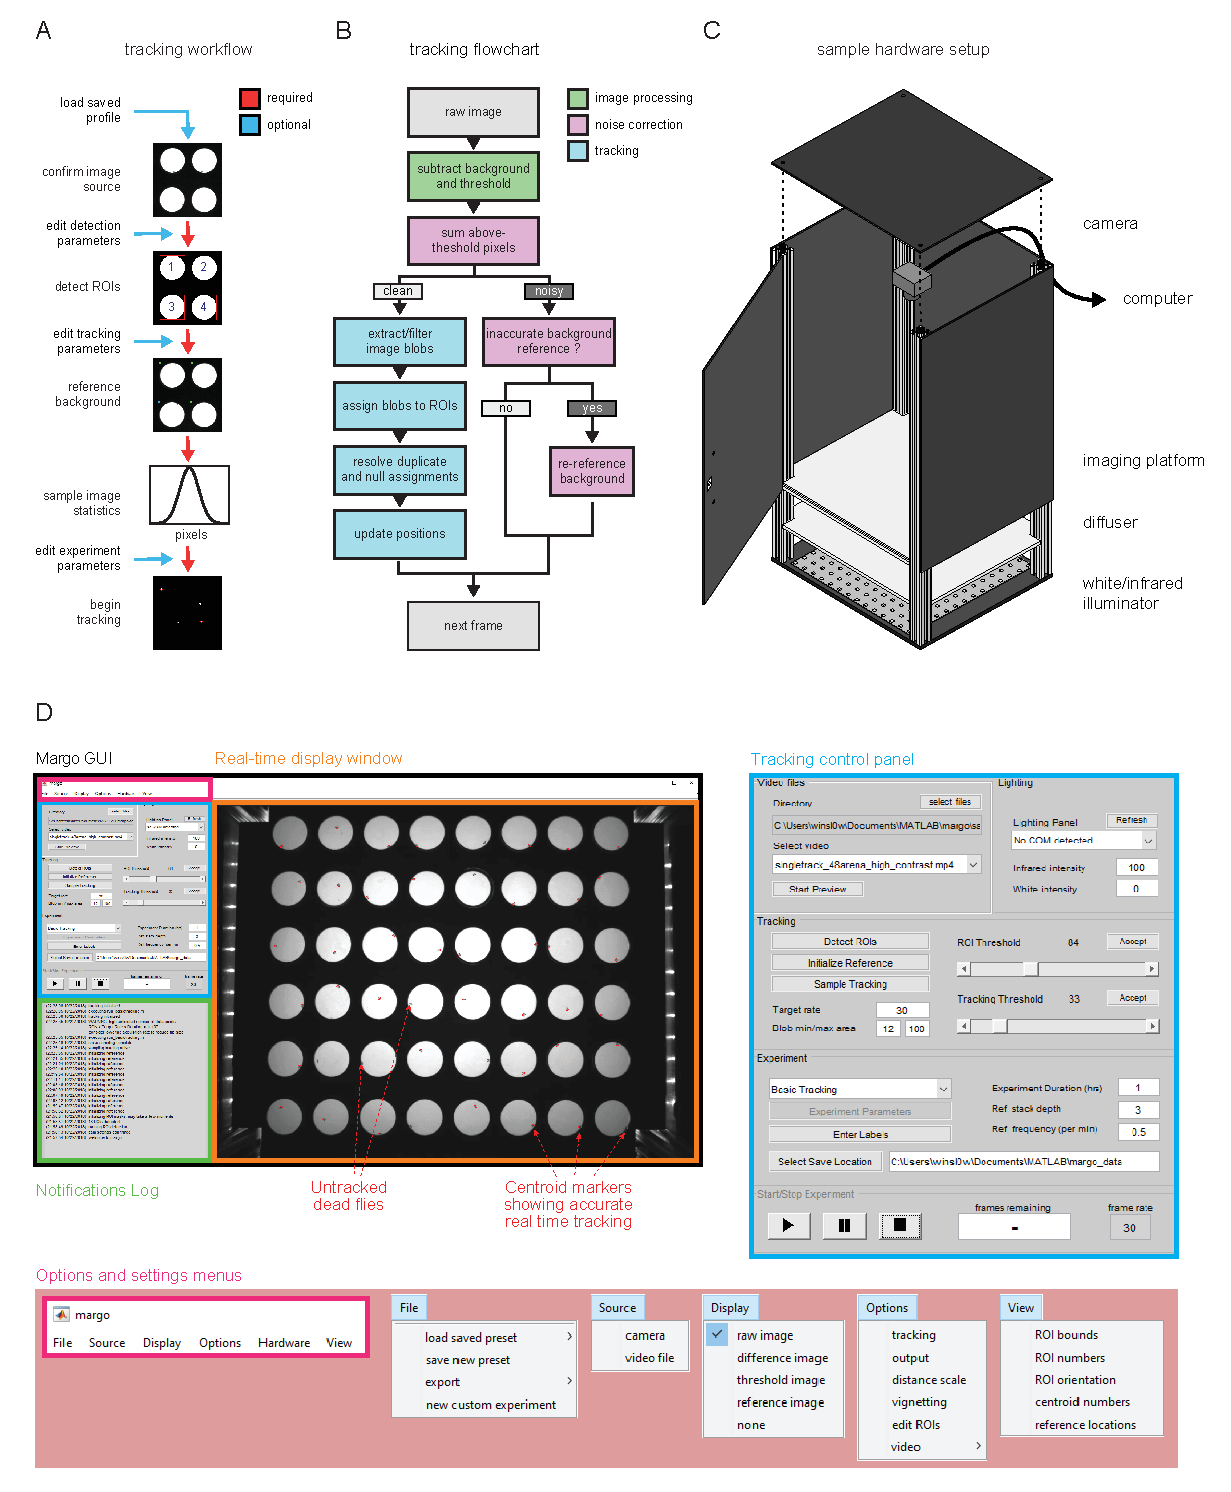
\includegraphics[width=0.9\textwidth]{../figures/autotracker_overview.pdf}
	\end{center}
	\caption*{\footnotesize \textbf{Figure 1. MARGO workflow, tracking algorithm, and sample behavioral box} -- A) Diagram of the user workflow to setup a new tracking experiment. Arrow color indicates whether the setup step is required. Before tracking, users define an input source, define ROIs to track, initialize a background image used to separate foreground and background, and sample the image statistics on a reference of clean tracking. Multiple points (blue arrows) are provided for customization of tracking parameters. B) Flowchart depicting the MARGO's frame-to-frame tracking routine. Each frame consists of image processing (green) to segment foreground from the background, noise estimation (magenta) to assess the quality of foreground segmentation and determine if the current frame can be tracked, and tracking (cyan) of foreground binary blobs. MARGO's tracking algorithm skips noisy frames and re-acquires the background image if many consecutive frames are deemed too noisy to track. C) Schematic of the behavioral boxes used to conduct tracking. Behavioral arenas are backlit with an LED illuminator and imaged with an overhead camera. The tracking camera is fitted with an infrared filter to allow light visible to the animals to be controlled independently of the tracking illumination. A diffuser panel between the LED backlight and the behavioral arenas is used to achieve even illumination. The camera and LED backlight are both connected to computer for real time tracking and control via MARGO. Such sophisticated imaging boxes are not required but help ensure consistent imaging quality.}
\end{figure}

\newpage
\begin{figure}[h!]
	\begin{center}
		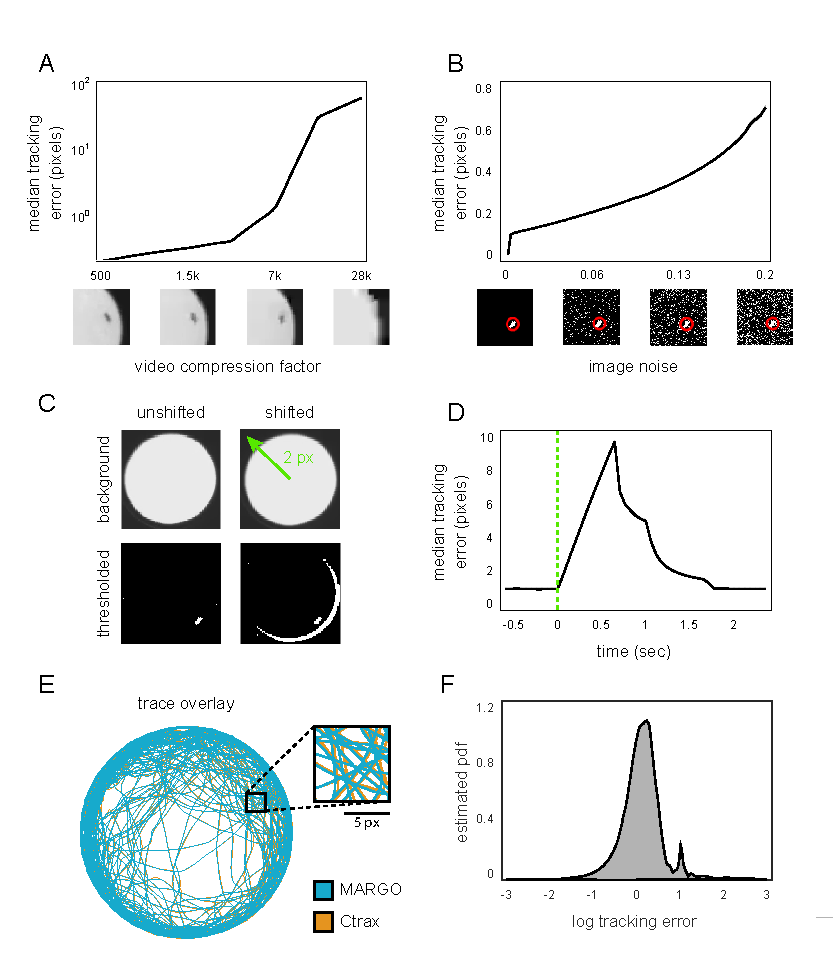
\includegraphics[width=0.9\textwidth]{../figures/autotracker_performance.pdf}
	\end{center}
	\caption*{\footnotesize \textbf{Figure 2. MARGO tracking accuracy and robustness to imaging noise} -- A) Median [refraf replace with mean] error of tracking performed on the same video at different levels of compression. Sample images of the same fly and frame are shown below. B) Median [refraf replace with mean] error of tracking performed on the same video with different levels of added noise. Pixel noise was manually added to the binary threshold image downstream of image processing and noise correction by converting any given pixel to true at a fixed probability (image noise). Sample images of the same fly and frame, as well as estimated position (red circle) are shown below. C) Diagram of the background image shifting scheme used to simulate background inaccuracy. D) Trial-triggered average tracking error centered on reference shifting. E-F) Sample trace comparison and log distribution of tracking error between traces acquired from the same video in both MARGO and Ctrax. The 95\% confidence interval of the above means were displayed but are within the thickness of lines.}
\end{figure}

\newpage
\begin{figure}[h!]
	\begin{center}
		\includegraphics[width=0.5\textwidth]{../figures/960_fly_imaging_panel_v2.pdf}
	\end{center}
	\caption*{\footnotesize \textbf{Figure 3. MARGO tracking throughput} - A) Image of the single-fly housing plates from the overhead tracking camera. B) Sample traces from a single fly on day 1 and day 6. Traces acquired on the first day appeared qualitatively similar to traces on the sixth day.  C) Raw speed data at three representative scales: heatmap of all individuals over the duration of the experiment (top), heatmap of all individuals from a sample three hour period (middle), raw speed traces from twenty individuals from a sample three minute period (bottom). Activity of most flies decreased over the six day duration. D) Individual kernel density estimates of log speed over the duration of the experiment. Column order was sorted by mean individual bout length in ascending order. E) Acquisition frame rate as a function of number of ROIs tracked in a simulated experiment. The acquisition rate decreased exponentially, consistent with a linear increase in inter-frame interval as a function of ROI number.}
\end{figure}

\newpage
\begin{figure}[h!]
	\begin{center}
		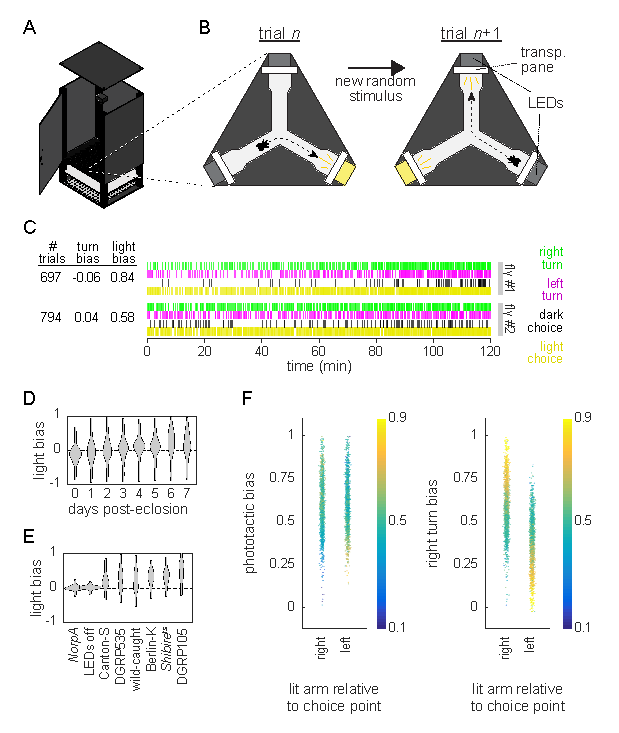
\includegraphics[width=0.9\textwidth]{../figures/LED_ymaze_panel.pdf}
	\end{center}
	\caption*{\footnotesize \textbf{Figure 4. High-throughput phototactic assay in Y-shaped arenas} -- A) Sample schematic of the LED Y-maze and behavioral box. B) Diagram of a single phototaxis maze and trial structure. New trials initiate by turning on (yellow) an LED in one of the two unoccupied maze arms. The trial ends when then animal turns into a new arm and the lit LED is turned off (gray). Each turn is scored for both handedness (left or right of the starting arm) and phototactic preference (positive or negative). C) Raw turn data for two sample flies. Each individual trial consists of both a phototactic and handedness choice. Individual means are typically averaged from hundreds of trials over a two hour period. D) Distribution of individual average phototactic biases for the same cohort of flies over the first 8 days post-eclosion. Horizontal dashed line indicates random bias at p=0.5. E) Comparison of individual average phototactic bias distributions for different wild-type fly lines. Blind flies (NorpA) and flies tested with all LEDs turned off (DGRP-105 dark) are included as negative controls.}
\end{figure}

\newpage
\begin{figure}[h!]
	\begin{center}
		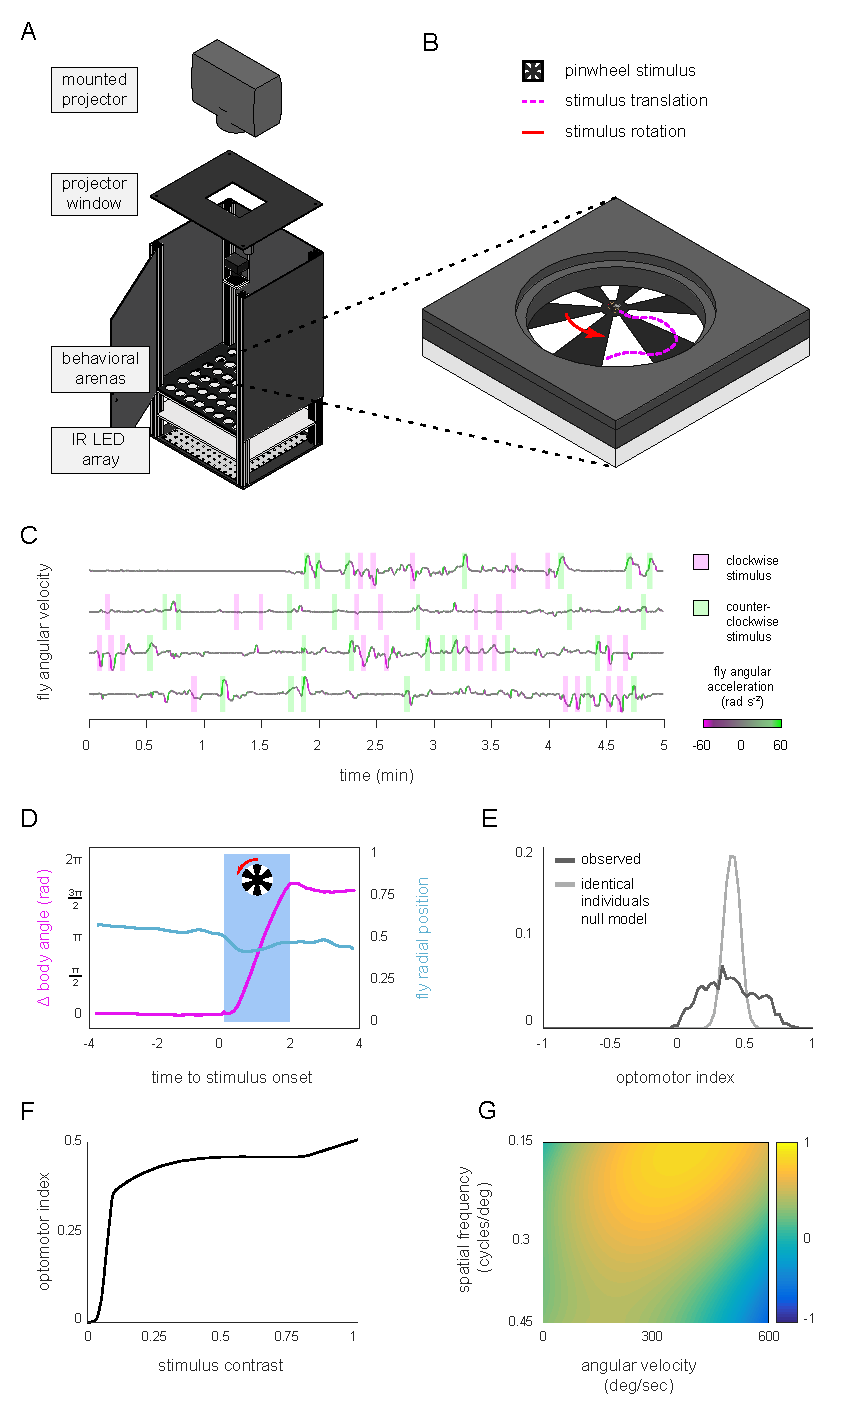
\includegraphics[width=0.5\textwidth]{../figures/Optomotor_panel.pdf}
	\end{center}
	\caption*{\footnotesize \textbf{Figure 5. High-throughput optomotor assay implementation in MARGO} -- A) Schematic of the optomotor arenas and behavioral box. B) Diagram of a single arena and optomotor stimulus. Trials begin with a pinwheel stimulus projected onto the center of mass of the fly. For each trial, the rotational direction (red arrow) of the stimulus is randomly chosen. The animal's tracked movement is used to maintain the stimulus center on estimated center of mass of the animal as it moves. Trials end when the stimulus is removed after a fixed duration (typically 2s). C) Sample raw individual time series data. Flies typically respond to optomotor stimuli by turning in the direction of the rotation of the stimulus. Hundreds of individual trials are recorded on average over a two hour period. D) Trial-triggered average optomotor response across all individuals. Change in body angle (magenta) is scored as positive or negative relative to the rotational direction of the stimulus. All trials were aligned to have change in body angle of zero at the onset of the stimulus. Average distance to the arena center (cyan) drops immediately preceeding stimulus onset due to the trial structure constraint that flies must be off the arena edge. E) Comparison of the observed distribution of individual average optomotor indices (n=1,860) to an identical individuals null model. The null model distributions were generated by bootstrap resampling trials from the shared distribution of all trials up to a maximum number randomly sampled from observed individual trial numbers. F) Population average optomor index as a function of normalized stimulus contrast. Pinwheel contrast was randomly varied on a trial-by-trial basis. G) Kernel density estimates of population average optomotor index as a function of stimulus spatial frequency and stimulus angular velocity. The 95\% confidence intervals of all above average traces are within the thickness of the line.}
\end{figure}

\newpage
\begin{figure}[t!]
	\begin{center}
		\vspace*{-8cm}
		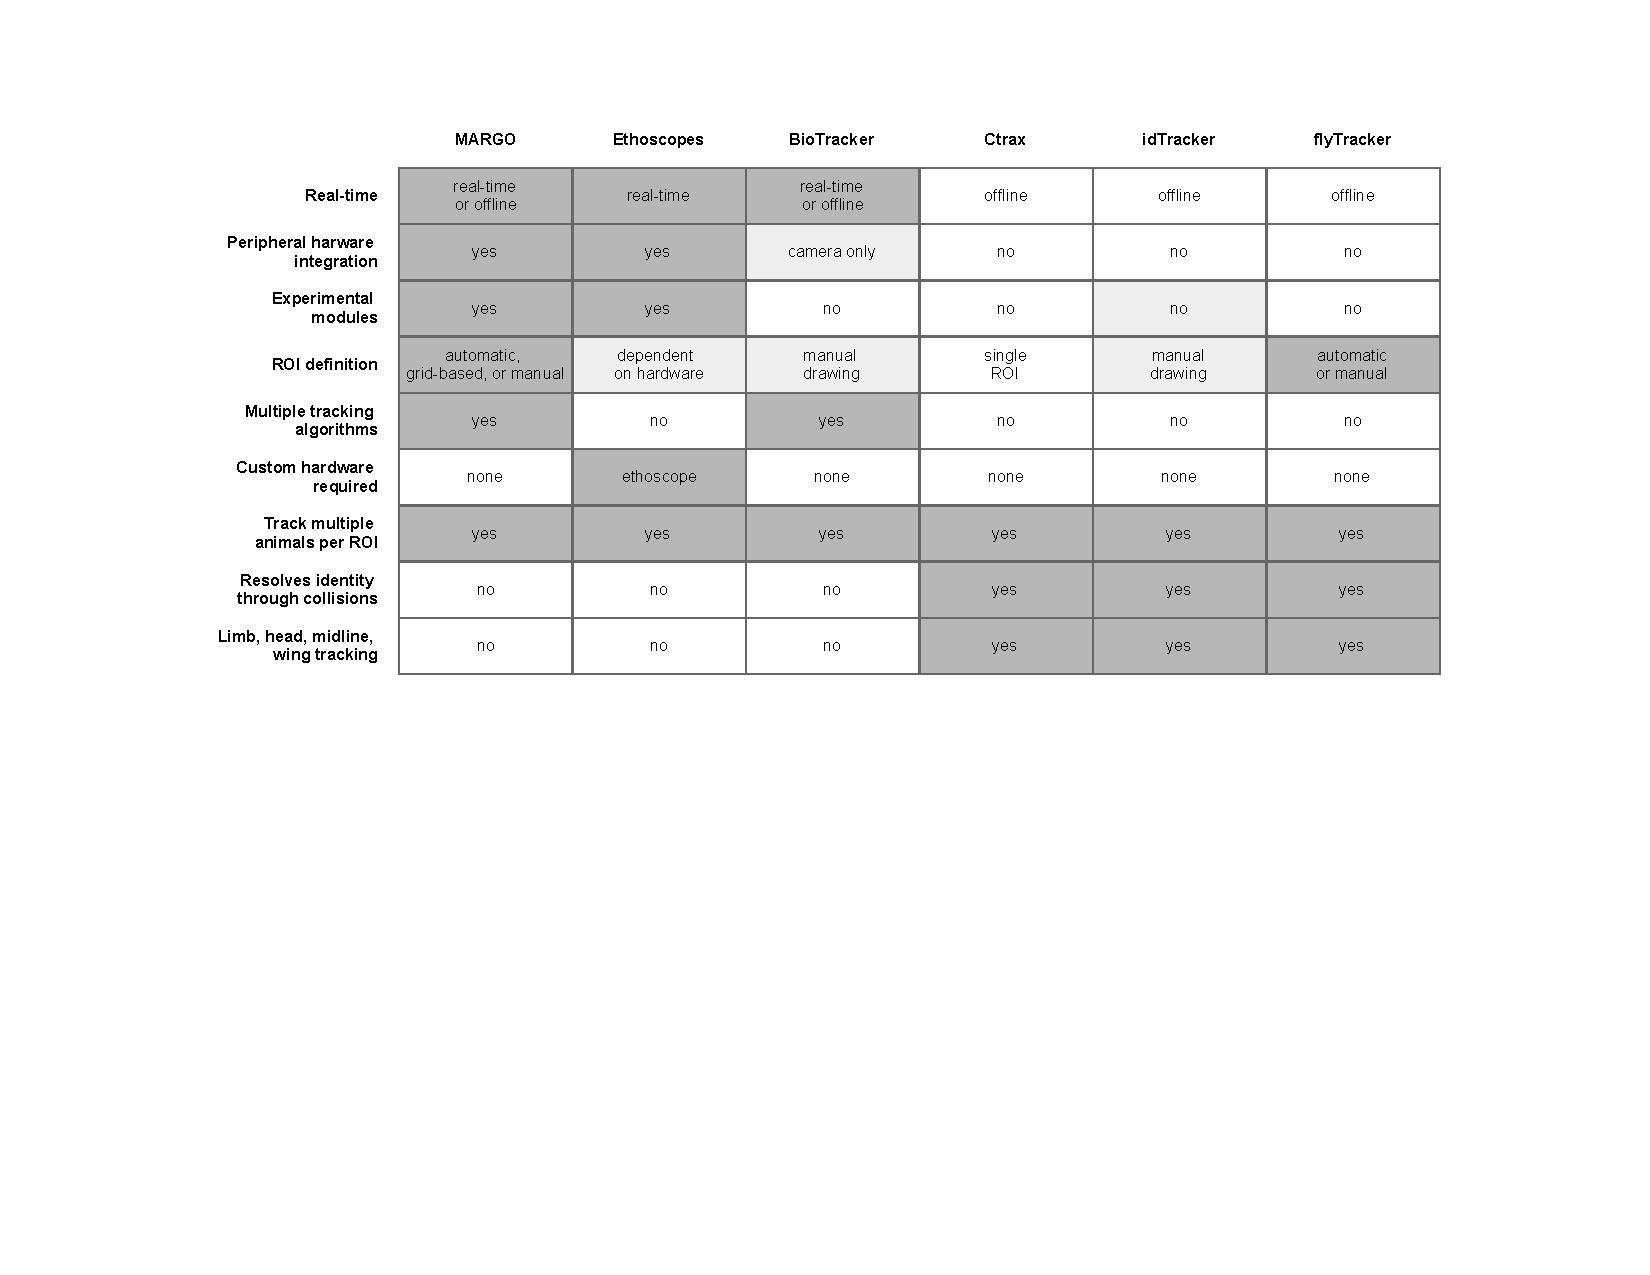
\includegraphics[width=0.9\textwidth]{../figures/platform_comparison_table.pdf}
	\end{center}
	\caption*{\footnotesize \textbf{Table 1. Comparison of open-source animal tracking packages} -- Existing software packages offer a variety of features useful to ethologists. We see trackers as falling into one of two broad categories: 1) real time trackers capable of very high-throughput with the potential hardware integration and stimulus delivery 2) off-line trackers capable of tracking postural features and maintaining individual identities without spatial segregation. We imagine MARGO, as well as other platforms such as Ethoscopes and BioTracker, falling into this first category. Experimental modules are a natural extension of real time trackers since tracking and other specialized components of experiments needs can be conducted in parallel. Popular examples of programs in the second category include Ctrax, idTracker, and flyTracker. The comparably more computationally expensive tracking algorithms used as well as the training and calibration process make them unsuitable for real time applications but offer the notable benefits of being able to study fine-scale postural and social behaviors.}
\end{figure}

\newpage
\begin{figure}[t!]
	\begin{center}
		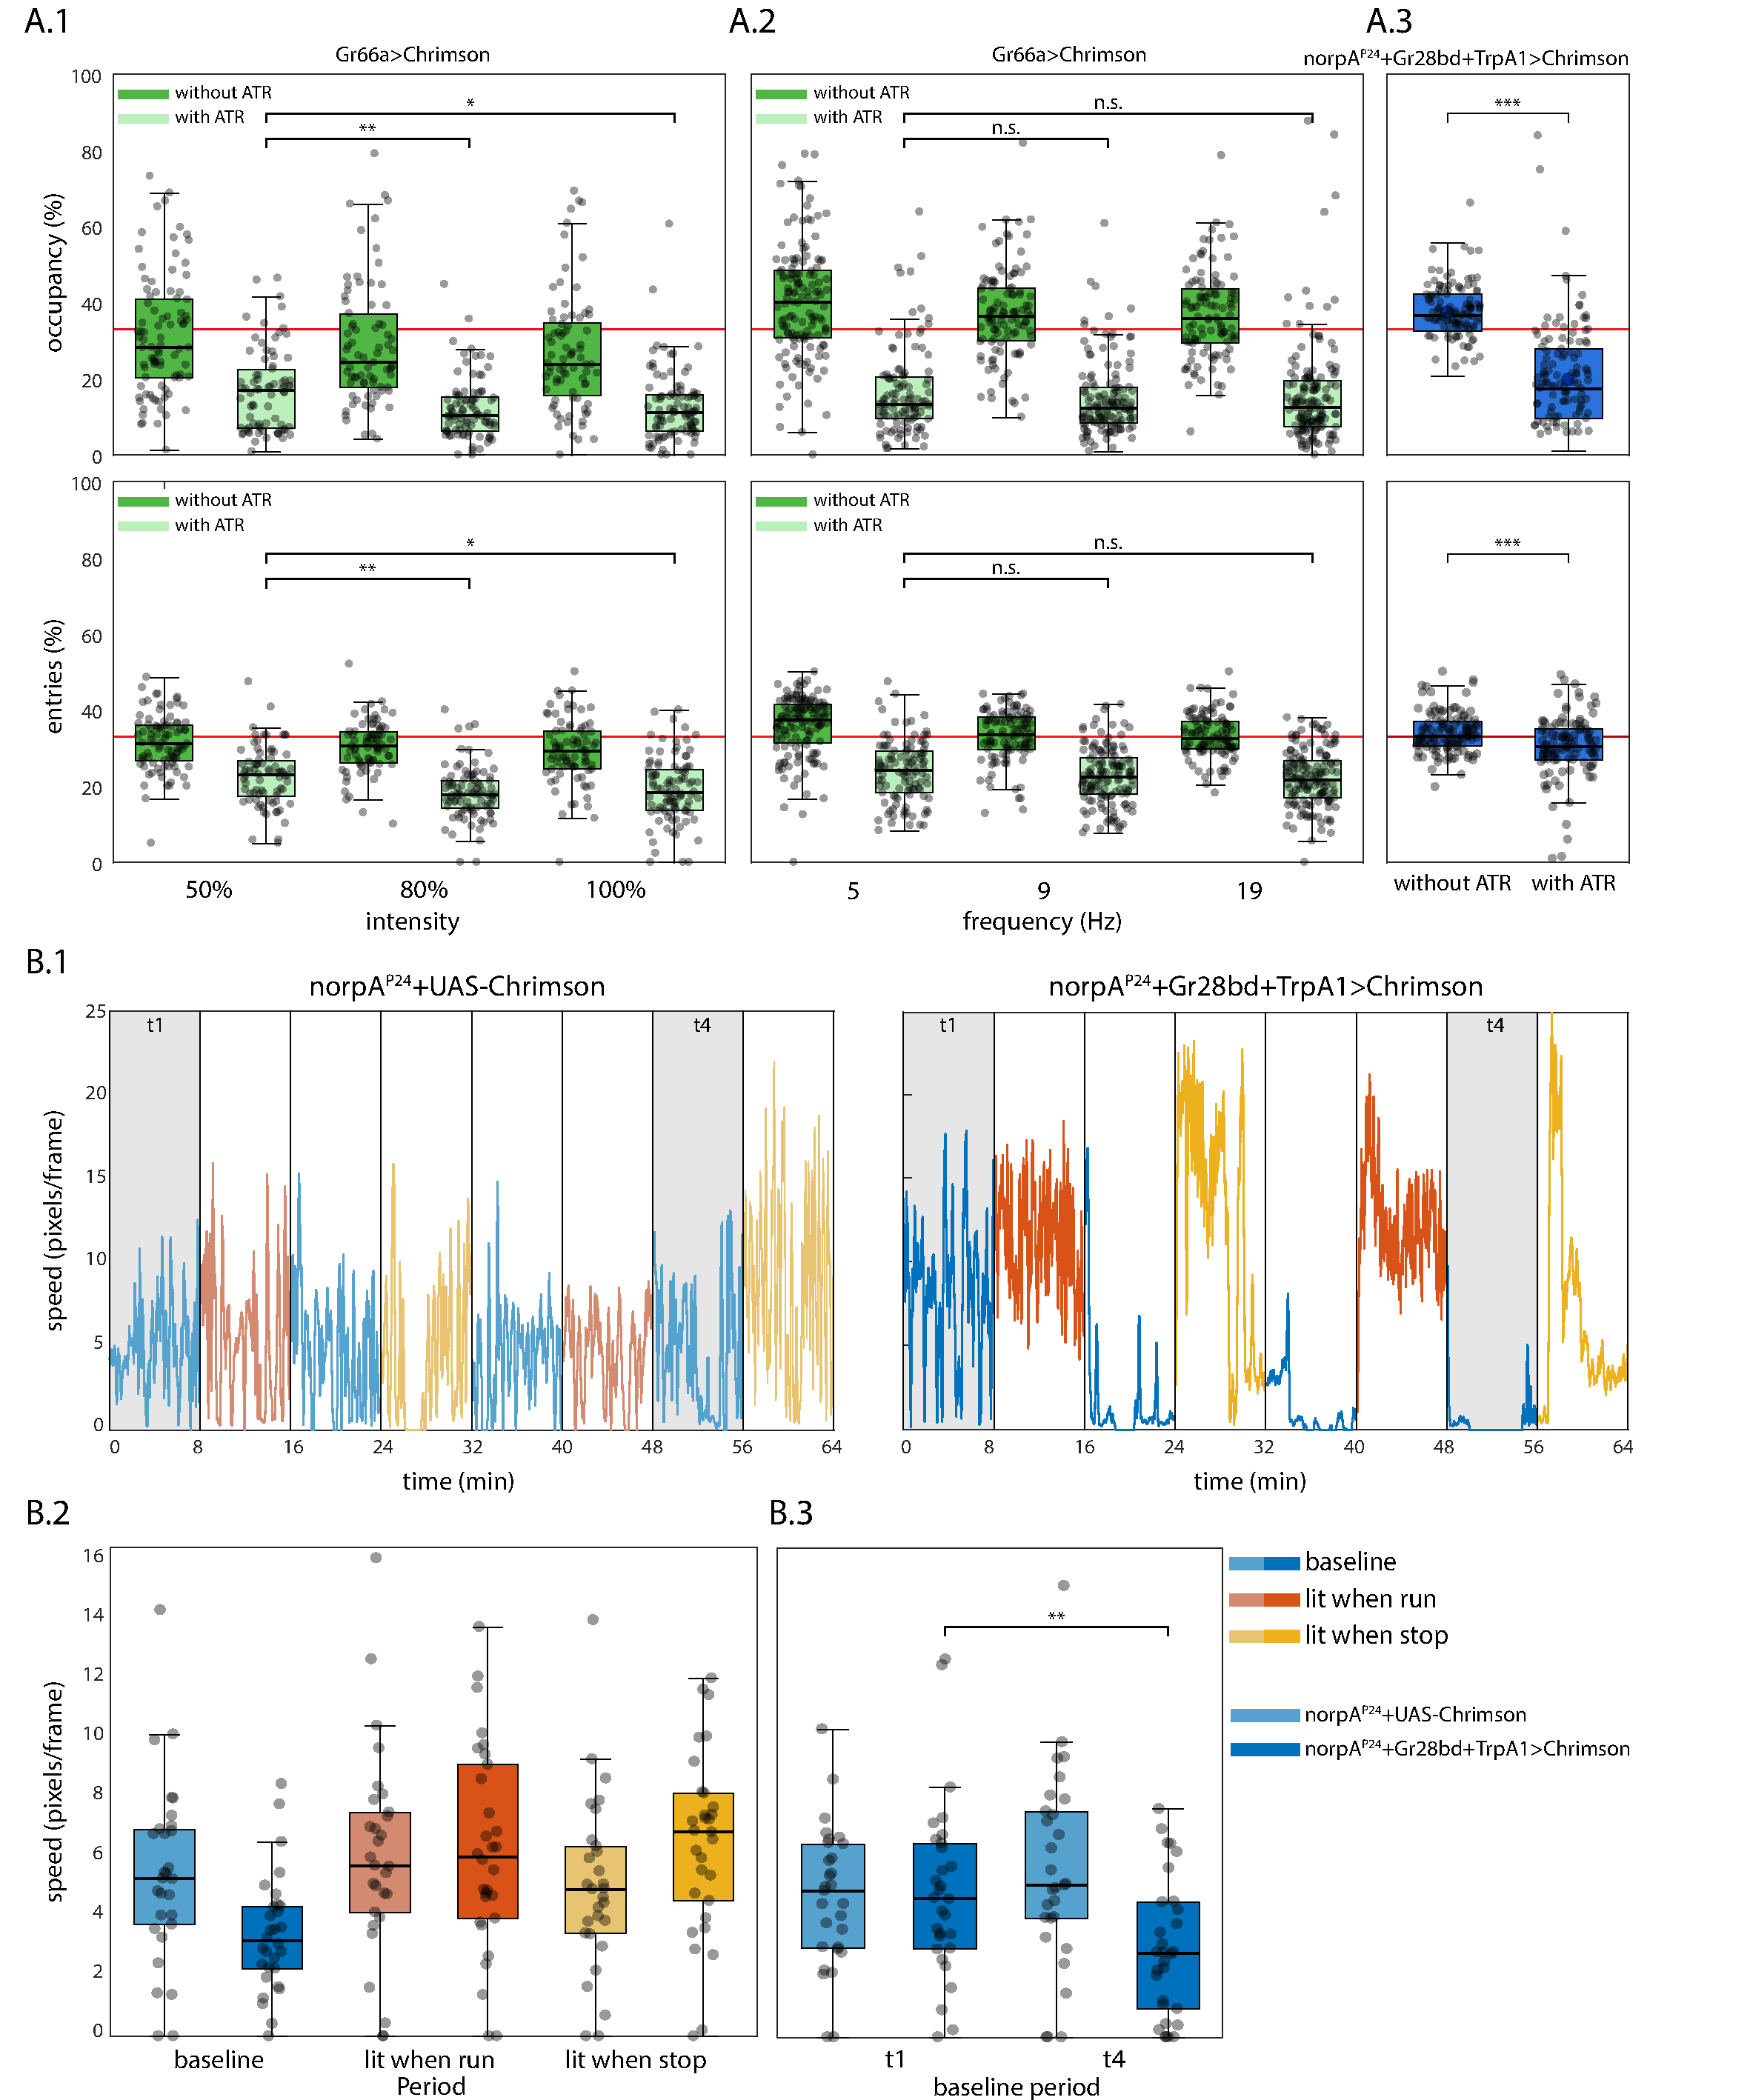
\includegraphics[width=0.6\textwidth]{../figures/optogenetics_fig.pdf}
	\end{center}
	\caption*{\footnotesize \textbf{Figure 6. Optogenetic closed-loop experiments with MARGO} -- A.1) Even at the lowest intensity (50\%), \textit{Gr66a>Chrimson} flies, expressing Chrimson in bitter-sensing neurons, fed with all-trans-retinal (ATR) in their food show a robust avoidance of the lit arm in a Y-Maze (compared to genetically identical flies not fed ATR), measured by the fraction of spent in the lit arm (occupancy, above) and by the fraction of arm-entries into the lit arm (entries, below). Increasing light intensity (x-axis) further decreases (slightly) the lit arm occupancy time and the lit arm entries even further.
	A.2) Even at the lowest frequency (5 Hz), \textit{Gr66a>Chrimson} flies fed ATR show a robust avoidance of the lit arm, compared to flies without ATR in the food, both in occupancy and in entries. Increasing the frequency further does not seem to increase the avoidance. P-values were calculated for key comparisons using a two-sample t-test, uncorrected for multiple comparisons; *:p<0.05, **:p<0.01, ***:p<0.001. 
	A.3) Blind \textit{norpA\textsuperscript{P24};Gr28bd+TrpA1>Chrimson} flies, expressing Chrimson in heat-sensitive neurons, also show decreased occupancy in the lit arm, whereas the fraction of entries into the lit arm appears unchanged compared to control flies not fed ATR. 
	Red lines at 33.3\% indicate equal preference for the lit arm compared to the other two arms of the Y-maze. Dots indicate scores from individual flies. 
	B.1) Example walking speed traces of an individual fly in circular arenas stimulated upon crossing a walking speed threshold. Color  indicates the eight consecutive experimental periods. Initial (b1) and final (b4) baseline periods are additionally marked with grey background. Speed is reported in pixels per frame (mm pixel^{-1}$\approx$1.7, seconds frame^{-1}$\approx$0.027).
	B.2) Compiled walking speed data for all periods and all flies. \textit{norpA\textsuperscript{P24};Gr28bd+TrpA1>Chrimson} flies increase their walking speed specifically during periods when stimulation is contingent on slow walking or resting (lit when stop), compared to lit when running periods and controls without the optogenetic effector \textit{norpA\textsuperscript{P24};UAS-Chrimson}.
	B.3) Walking speed during the initial baseline period did not differ between experimental and control flies (t1). In contrast, after three contingent stimulation periods, walking speed in experimental flies was significantly lower than in control flies (t4). 
	All flies in B were fed with all-trans-retinal.} 
\end{figure}

\end{document}